\documentclass{beamer}\usepackage[]{graphicx}\usepackage[]{xcolor}
% maxwidth is the original width if it is less than linewidth
% otherwise use linewidth (to make sure the graphics do not exceed the margin)
\makeatletter
\def\maxwidth{ %
  \ifdim\Gin@nat@width>\linewidth
    \linewidth
  \else
    \Gin@nat@width
  \fi
}
\makeatother

\definecolor{fgcolor}{rgb}{0.345, 0.345, 0.345}
\newcommand{\hlnum}[1]{\textcolor[rgb]{0.686,0.059,0.569}{#1}}%
\newcommand{\hlstr}[1]{\textcolor[rgb]{0.192,0.494,0.8}{#1}}%
\newcommand{\hlcom}[1]{\textcolor[rgb]{0.678,0.584,0.686}{\textit{#1}}}%
\newcommand{\hlopt}[1]{\textcolor[rgb]{0,0,0}{#1}}%
\newcommand{\hlstd}[1]{\textcolor[rgb]{0.345,0.345,0.345}{#1}}%
\newcommand{\hlkwa}[1]{\textcolor[rgb]{0.161,0.373,0.58}{\textbf{#1}}}%
\newcommand{\hlkwb}[1]{\textcolor[rgb]{0.69,0.353,0.396}{#1}}%
\newcommand{\hlkwc}[1]{\textcolor[rgb]{0.333,0.667,0.333}{#1}}%
\newcommand{\hlkwd}[1]{\textcolor[rgb]{0.737,0.353,0.396}{\textbf{#1}}}%
\let\hlipl\hlkwb

\usepackage{framed}
\makeatletter
\newenvironment{kframe}{%
 \def\at@end@of@kframe{}%
 \ifinner\ifhmode%
  \def\at@end@of@kframe{\end{minipage}}%
  \begin{minipage}{\columnwidth}%
 \fi\fi%
 \def\FrameCommand##1{\hskip\@totalleftmargin \hskip-\fboxsep
 \colorbox{shadecolor}{##1}\hskip-\fboxsep
     % There is no \\@totalrightmargin, so:
     \hskip-\linewidth \hskip-\@totalleftmargin \hskip\columnwidth}%
 \MakeFramed {\advance\hsize-\width
   \@totalleftmargin\z@ \linewidth\hsize
   \@setminipage}}%
 {\par\unskip\endMakeFramed%
 \at@end@of@kframe}
\makeatother

\definecolor{shadecolor}{rgb}{.97, .97, .97}
\definecolor{messagecolor}{rgb}{0, 0, 0}
\definecolor{warningcolor}{rgb}{1, 0, 1}
\definecolor{errorcolor}{rgb}{1, 0, 0}
\newenvironment{knitrout}{}{} % an empty environment to be redefined in TeX

\usepackage{alltt}
\usepackage{graphicx}
% \usepackage{comment}

\usepackage{graphicx}
\usepackage{verbatim}
\usepackage{etoolbox}
\usepackage{everysel}
% \usepackage{enumitem}

%% This package allows text highlighting
\usepackage{soul}

%% This sets the theme of the presentation which controls
%% the formatting of the slides
\usetheme{Boadilla}

%% Turn off the navigation symbols
\setbeamertemplate{navigation symbols}{} 

%% Change the default itemize [ball]s to [circle]s
\setbeamertemplate{itemize items}[circle]

%% Change the default enumerate [ball]s to plain text
\setbeamertemplate{enumerate items}[default]

%% Load the enumitem package and ensure it works nicely with beamer
% \setitemize{label=\usebeamerfont*{itemize item}
%   \usebeamercolor[fg]{itemize item}
%   \usebeamertemplate{itemize item}}
% \setenumerate{label=\usebeamerfont*{enumerate item}
%   \usebeamercolor[fg]{enumerate item}
%   \usebeamertemplate{enumerate item}}

%% Set the author block so STATS 201/8 appears on every
\author{STATS 201/8}

%% Clear the date block
\date{}


\setbeamercolor{title}{bg=blue!40}
\setbeamerfont{title}{size=\LARGE,series=\bfseries}

%%Sectioning commands
\setbeamercolor{section title}{bg=blue!20}
\setbeamerfont{section title}{size=\large}

\setbeamertemplate{section page}{%
    \begingroup
        \begin{beamercolorbox}[sep=10pt,center,rounded=true,shadow=true]{section title}
        \usebeamerfont{section title}Section~\thechapter.\thesection \newline \insertsection\par
        \end{beamercolorbox}
		\vfill
    \endgroup
}

\newcommand{\BeginSection}[1]{\section{#1} \frame{\sectionpage}}
%\AtBeginSection[]{%
%    \begin{frame}
%        \sectionpage
%    \end{frame}
%}


%% This makes all equations blue
\AtBeginEnvironment{equation*}{\color{blue}}
\AtBeginEnvironment{align*}{\color{blue}}
\everymath{\color{blue}}

%% This puts a 0 point space between paragraphs, means we don't need to use vspace, or list environments if 
%% we don't want to
\setlength{\parskip}{0pt}


%% Russell: removes spaces after R input/output?
\setlength{\topsep}{0.5mm}

%% David: In addition to Russel's command to remove spaces after R input/output, these commands remove the space between R input/output.
%% Stackoverflow link: https://stackoverflow.com/questions/35734525/reduce-space-between-code-chunks-and-code-output-in-rmarkdown-beamer-presentatio
%% \setlength{\OuterFrameSep}{-2pt}
\makeatletter
\preto{\@verbatim}{\topsep=-1pt \partopsep=-1pt }
\makeatother

%% Some useful colors
\definecolor{darkgreen}{rgb}{0.176,0.486,0.031}
\definecolor{redbrown}{HTML}{950605}
\definecolor{darkred}{HTML}{d80605}


%% nice little macro for changing the font of R code
\newcommand{\rcode}[1]{\protect{\color{darkgreen}\texttt{#1}}}

%% macro for bold blue italics
\newcommand{\blueBoldEmph}[1]{{\color{blue}\textbf{\emph{#1}}}}

% ~iid macro
\newcommand{\iid }{\stackrel{iid}{\sim}}

%% Macro for t-test amd P-value
\newcommand{\ttest}{\emph{t}-test}
\newcommand{\pval}{\emph{P}-value}

%% Statistics operators 
\DeclareMathOperator{\Bias}{Bias}
\DeclareMathOperator{\Cov}{Cov}
\DeclareMathOperator*{\Cor}{Cor}
\DeclareMathOperator{\E}{E}
\DeclareMathOperator{\MSE}{MSE}
\DeclareMathOperator{\Odds}{Odds}
\DeclareMathOperator{\OR}{OR}
\DeclareMathOperator{\PMSE}{PMSE}
\DeclareMathOperator{\sd}{sd}
\DeclareMathOperator{\se}{se}
\DeclareMathOperator*{\Var}{Var}
\DeclareMathOperator{\logit}{logit}

%% Should see if can make this a mathop
\newcommand{\comb}[2]{\mbox{$\big(_{#2}^{#1}\big)$}}






\IfFileExists{upquote.sty}{\usepackage{upquote}}{}
\begin{document}
\newcommand{\thechapter}{7}
%\SweaveOpts{concordance=TRUE}

\title{Chapter 7: \\ Power law linear models}
\institute{University of Auckland}


\begin{frame}
\titlepage
\end{frame}


\begin{frame}[t]
\frametitle{Learning Outcomes}
In this chapter you will learn about:
\begin{center}
\vspace{16pt}
\begin{minipage}{0.9\textwidth}
  \begin{itemize}
  \item Power law models 
  \item How to interpret the effect of the explanatory variable
  \item Relevant \rcode{R}-code.
  \end{itemize}
\end{minipage}
\end{center}
\end{frame}


%%%%%%%%%%%%%%%%%%%%%%%%%%%%%%%%%%%%%%%%%%%%%%%%%%%%%%%%%%%%%%%%%%%%%%%%%%%%%%%%%%%%%%%%%%%
\BeginSection{Power law model example}
%%%%%%%%%%%%%%%%%%%%%%%%%%%%%%%%%%%%%%%%%%%%%%%%%%%%%%%%%%%%%%%%%%%%%%%%%%%%%%%%%%%%%%%%%%%


\begin{frame}
\frametitle{Example -- Weight of snapper as a function of length}

Those of you who fish in the Hauraki Gulf will know that the minimum legal size for
retaining a snapper is 30 cm.
Here, we want to use snapper length to explain snapper weight, and in particular
we want to estimate the weight of 30 cm snapper.

\begin{columns}
\begin{column}{0.45\textwidth}
Note that this research question is highly relevant, 
since the relationship between length and weight is crucial for the 
stock assessments of snapper.
\end{column}
\begin{column}{0.55\textwidth}
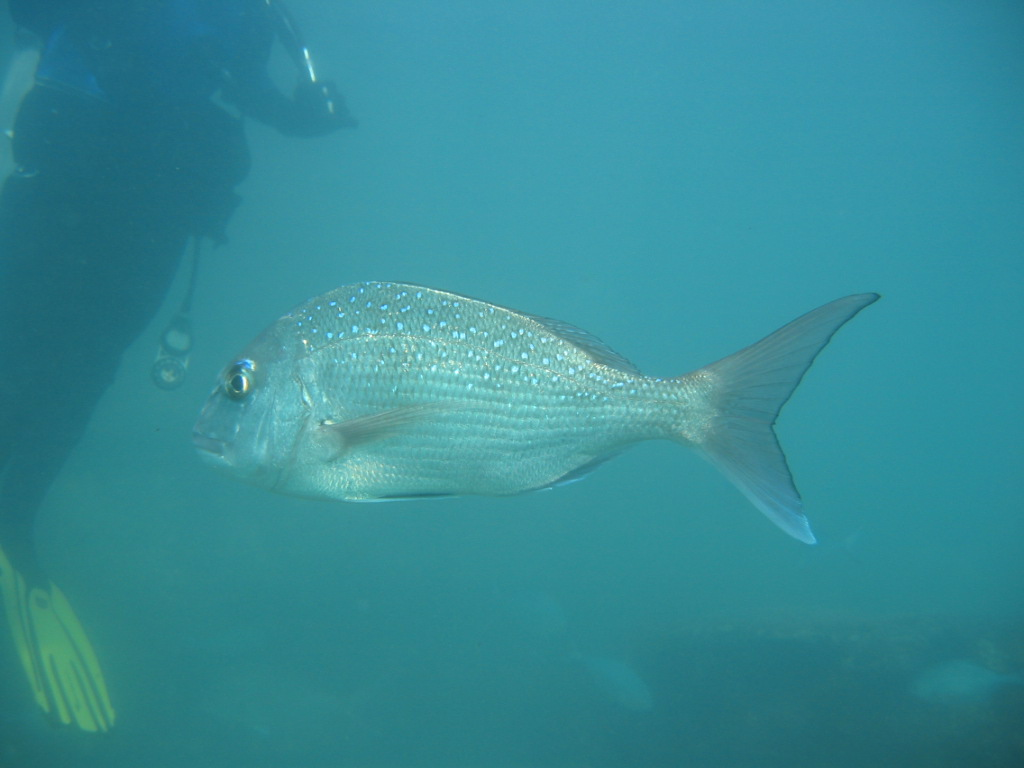
\includegraphics[width=2.5in]{SnapperAtLeigh.jpg}
\end{column}
\end{columns}
\end{frame}


\begin{frame}[fragile]
\frametitle{Weight of snapper as a function of length}
What does our intuition tell us about the shape of the relationship between length and weight?
\bigskip
\begin{itemize}\setlength{\itemsep}{5mm}
\item Straight line?
\item Quadratic?
\item Exponential?
\item Other?
\end{itemize}
\end{frame}


\begin{frame}[fragile]
\frametitle{Weight of snapper as a function of length\ldots}
The data file \rcode{SnapWgt.txt} contains measurements on 844 snapper.
The variables are:

\begin{center}
\begin{tabular}{lp{15cm}}
\rcode{len} & fork length (cm) \\
\rcode{wgt} & weight (kg)
\end{tabular}
\end{center}

\begin{knitrout}\scriptsize
\definecolor{shadecolor}{rgb}{0.969, 0.969, 0.969}\color{fgcolor}\begin{kframe}
\begin{alltt}
\hlstd{> }\hlstd{Snap.df}\hlkwb{=}\hlkwd{read.table}\hlstd{(}\hlstr{"SnapWgt.txt"}\hlstd{,}\hlkwc{header}\hlstd{=}\hlnum{TRUE}\hlstd{)}
\hlstd{> }\hlkwd{plot}\hlstd{(wgt}\hlopt{~}\hlstd{len,}\hlkwc{data}\hlstd{=Snap.df,}\hlkwc{xlab}\hlstd{=}\hlstr{"Length (cm)"}\hlstd{,}\hlkwc{ylab}\hlstd{=}\hlstr{"Weight (kg)"}\hlstd{)}
\end{alltt}
\end{kframe}
\end{knitrout}

\end{frame}


\begin{frame}[fragile]
\frametitle{Weight of snapper as a function of length\ldots}


\begin{figure}
  \centering
  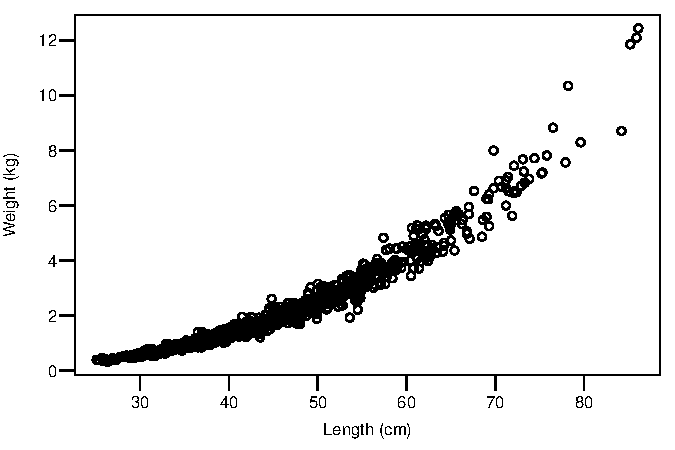
\includegraphics{figure/RC-H07-002}
\end{figure}

\end{frame}


\begin{frame}[fragile]
\frametitle{Weight of snapper as a function of length\ldots}
Clearly there is a non-linear relationship between weight and length.\\
\medskip
Geometry tells us that if an object changes in overall size while keeping the
same shape (i.e., same ratio between height, depth and length), 
then its volume will increase with the 3rd power of length.\\
\medskip
\begin{itemize}
\item For a cube with sides of length $l$, $volume=len^3$.
\item For a sphere with radius $r$, $volume=\frac{4}{3}\pi r^3$.
\end{itemize}
\medskip
That is, $volume \propto len^3$. In other words
\[ 
volume = k_1 \times len^3 
\]
for some constant $k_1$.\\
\medskip
Assuming weight of a solid object is proportional to its volume, we conclude
\[ 
weight = \alpha \times len^3
\]
for some constant $\alpha$.
\end{frame}


\begin{frame}[fragile]
\frametitle{Weight of snapper as a function of length\ldots}
Those of you who have caught snapper will know that they do exhibit a small change 
in shape as they grow larger, so it would be better to use the model
\[ 
weight = \alpha \times len^{\beta_1} 
\]
where $\beta_1$ is some constant that may be close to, but not necessarily equal to 3.\\
\medskip
Taking logs gives
\[ \log(weight) = \log(\alpha) + \beta_1 \times \log(len) \]
which we can rewrite as
\[ \log(weight) = \beta_0 +\beta_1 \times \log(len) \ . \]
\end{frame}


\begin{frame}[fragile]
\frametitle{Weight of snapper as a function of length\ldots}
The formula on the previous slide specifies an assumed (i.e, expected) relationship between
$\log(weight)$ and $\log(len)$ of a snapper.\\
\medskip
Of course, snapper of a given length will have some variability in their weight,
just as humans of a given height vary in their weight.
So, what we are really saying is that the weight (kg) of an individual snapper of length $len$ (cm)
is
\[
\log(weight) = \beta_0 +\beta_1 \times \log(len) + \varepsilon 
\]
where $\varepsilon$ is some random variability (i.e., error around the expected value).

\medskip

The above formula should be of very familiar form to you by now. 
Provided that we make the assumption that $\varepsilon \sim N(0,\sigma^2)$ then this is precisely
the simple linear regression model with response variable $\log(weight)$ and
explanatory variable $\log(len)$.
\end{frame}


\begin{frame}[fragile]
\frametitle{Weight of snapper as a function of length\ldots}
\framesubtitle{Fitting a simple linear model using log(weight) and log(length)}
Let us look at the relationship between log(wgt) and log(len)

\begin{knitrout}\scriptsize
\definecolor{shadecolor}{rgb}{0.969, 0.969, 0.969}\color{fgcolor}\begin{kframe}
\begin{alltt}
\hlstd{> }\hlkwd{plot}\hlstd{(}\hlkwd{log}\hlstd{(wgt)}\hlopt{~}\hlkwd{log}\hlstd{(len),}\hlkwc{data}\hlstd{=Snap.df,}\hlkwc{xlab}\hlstd{=}\hlstr{"log(Length)"}\hlstd{,}\hlkwc{ylab}\hlstd{=}\hlstr{"log(Weight)"}\hlstd{)}
\end{alltt}
\end{kframe}
\end{knitrout}



\begin{figure}
  \centering
  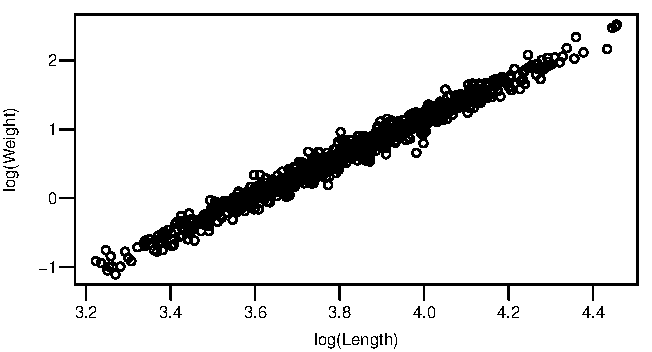
\includegraphics{figure/RC-H07-004}
\end{figure}

Looking good.
\end{frame}


\begin{frame}[fragile]
\frametitle{Weight of snapper as a function of length\ldots}
\framesubtitle{Fitting a simple linear model using log(weight) and log(length)\ldots}

\begin{knitrout}\scriptsize
\definecolor{shadecolor}{rgb}{0.969, 0.969, 0.969}\color{fgcolor}\begin{kframe}
\begin{alltt}
\hlstd{> }\hlstd{Snap.lm}\hlkwb{=}\hlkwd{lm}\hlstd{(}\hlkwd{log}\hlstd{(wgt)}\hlopt{~}\hlkwd{log}\hlstd{(len),}\hlkwc{data}\hlstd{=Snap.df)}
\hlstd{> }\hlkwd{plot}\hlstd{(Snap.lm,}\hlkwc{which}\hlstd{=}\hlnum{1}\hlstd{)}
\end{alltt}
\end{kframe}
\end{knitrout}



\begin{figure}
  \centering
  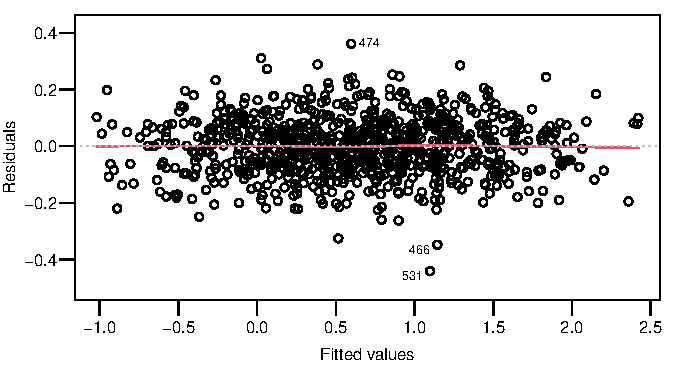
\includegraphics{figure/RC-H07-006}
\end{figure}

\end{frame}


\begin{frame}[fragile]
\frametitle{Weight of snapper as a function of length\ldots}
\framesubtitle{Fitting a simple linear model using log(weight) and log(length)\ldots}

Check the Normality assumption.
\begin{knitrout}\scriptsize
\definecolor{shadecolor}{rgb}{0.969, 0.969, 0.969}\color{fgcolor}\begin{kframe}
\begin{alltt}
\hlstd{> }\hlkwd{normcheck}\hlstd{(Snap.lm)}
\end{alltt}
\end{kframe}
\end{knitrout}



\begin{figure}
  \centering
  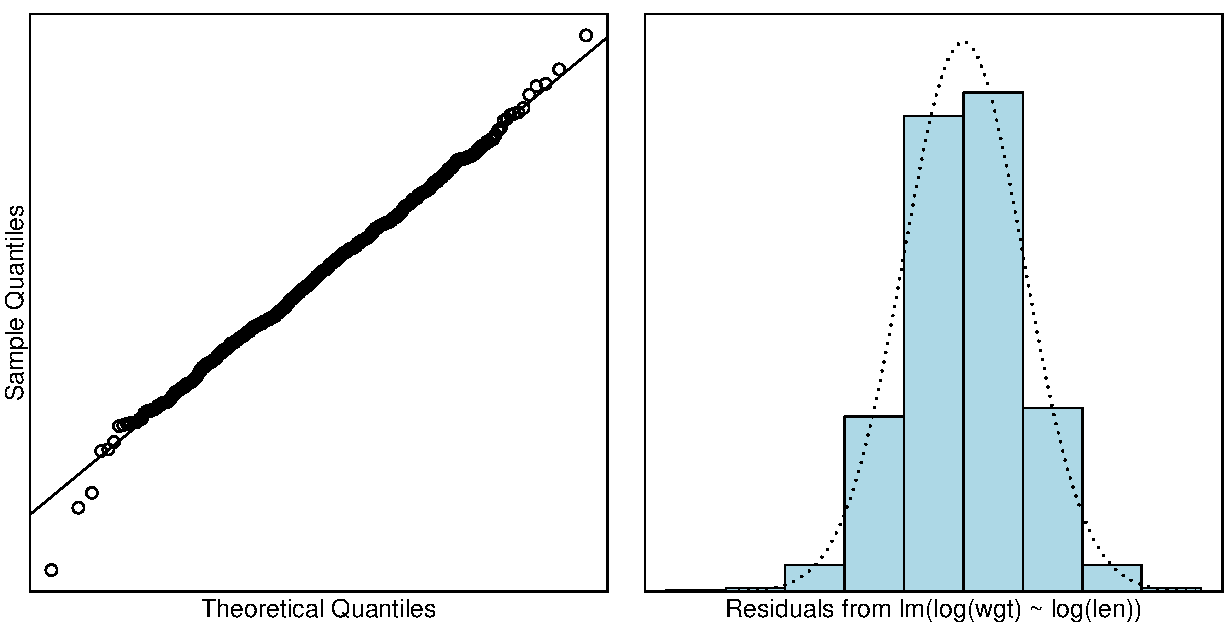
\includegraphics[scale=0.5]{figure/RC-H07-008}
\end{figure}

% No worries.
\end{frame}

\begin{frame}[fragile]
\frametitle{Weight of snapper as a function of length\ldots}
\framesubtitle{Fitting a simple linear model using log(weight) and log(length)\ldots}

Check for influential observations.
\begin{knitrout}\scriptsize
\definecolor{shadecolor}{rgb}{0.969, 0.969, 0.969}\color{fgcolor}\begin{kframe}
\begin{alltt}
\hlstd{> }\hlkwd{cooks20x}\hlstd{(Snap.lm)}
\end{alltt}
\end{kframe}
\end{knitrout}



\begin{figure}
  \centering
  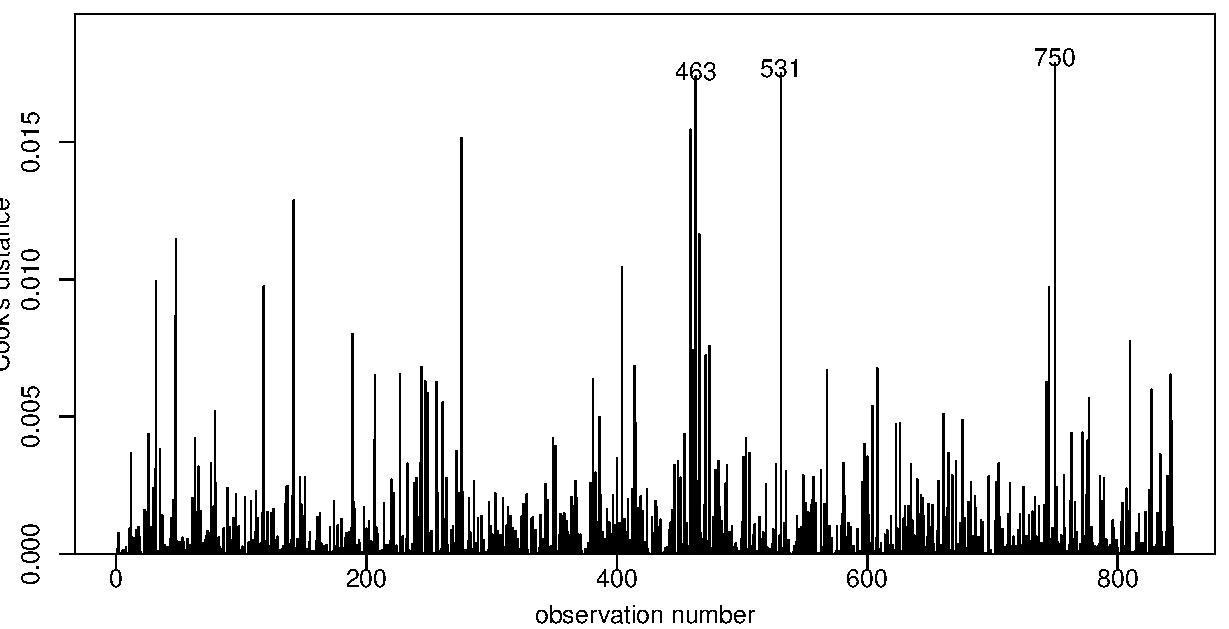
\includegraphics[scale=0.5]{figure/RC-H07-010}
\end{figure}

\end{frame}



\begin{frame}[fragile]
\frametitle{Weight of snapper as a function of length\ldots}
\framesubtitle{Making inference}
We can trust the fitted model.

\begin{knitrout}\scriptsize
\definecolor{shadecolor}{rgb}{0.969, 0.969, 0.969}\color{fgcolor}\begin{kframe}
\begin{alltt}
\hlstd{> }\hlkwd{summary}\hlstd{(Snap.lm)}
\end{alltt}
\end{kframe}
\end{knitrout}
\begin{knitrout}\scriptsize
\definecolor{shadecolor}{rgb}{0.969, 0.969, 0.969}\color{fgcolor}\begin{kframe}
\begin{verbatim}
Coefficients:
             Estimate Std. Error t value Pr(>|t|)    
(Intercept) -10.01416    0.05602  -178.7   <2e-16 ***
log(len)      2.79104    0.01469   190.0   <2e-16 ***
---
Residual standard error: 0.1012 on 842 degrees of freedom
Multiple R-squared:  0.9772,	Adjusted R-squared:  0.9772 
F-statistic: 3.609e+04 on 1 and 842 DF,  p-value: < 2.2e-16
\end{verbatim}
\begin{alltt}
\hlstd{> }\hlkwd{confint}\hlstd{(Snap.lm)}
\end{alltt}
\begin{verbatim}
                 2.5 %    97.5 %
(Intercept) -10.124126 -9.904199
log(len)      2.762204  2.819879
\end{verbatim}
\end{kframe}
\end{knitrout}
\end{frame}



\begin{frame}[fragile]
\frametitle{Weight of snapper as a function of length\ldots}
\framesubtitle{The fitted line on the log scale}

\begin{knitrout}\scriptsize
\definecolor{shadecolor}{rgb}{0.969, 0.969, 0.969}\color{fgcolor}\begin{kframe}
\begin{alltt}
\hlstd{> }\hlkwd{plot}\hlstd{(}\hlkwd{log}\hlstd{(wgt)}\hlopt{~}\hlkwd{log}\hlstd{(len),}\hlkwc{data}\hlstd{=Snap.df,}\hlkwc{xlab}\hlstd{=}\hlstr{"log(Length)"}\hlstd{,}\hlkwc{ylab}\hlstd{=}\hlstr{"log(Weight)"}\hlstd{)}
\hlstd{> }\hlkwd{abline}\hlstd{(}\hlkwd{coef}\hlstd{(Snap.lm),}\hlkwc{lty}\hlstd{=}\hlnum{5}\hlstd{,} \hlkwc{col}\hlstd{=}\hlstr{"red"}\hlstd{)}
\end{alltt}
\end{kframe}
\end{knitrout}



\begin{figure}
  \centering
  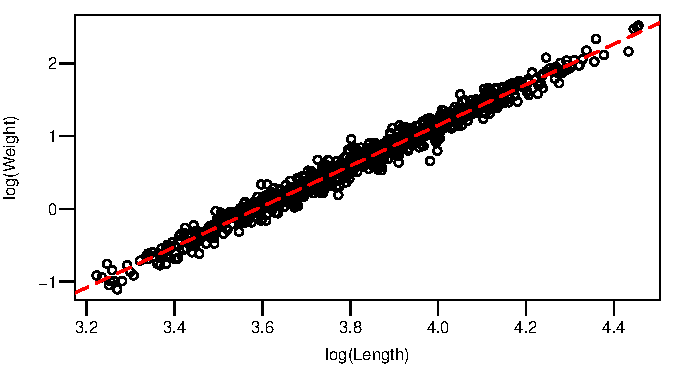
\includegraphics{figure/RC-H07-014}
\end{figure}

\end{frame}


\begin{frame}[fragile]
\frametitle{Weight of snapper as a function of length\ldots}
\framesubtitle{The fitted line on the log scale\ldots}

Let us redo the plot on the raw scale (rather than log scale):
\begin{knitrout}\scriptsize
\definecolor{shadecolor}{rgb}{0.969, 0.969, 0.969}\color{fgcolor}\begin{kframe}
\begin{alltt}
\hlstd{> }\hlkwd{plot}\hlstd{(wgt}\hlopt{~}\hlstd{len,} \hlkwc{data} \hlstd{= Snap.df)}
\hlstd{> }\hlstd{pred.df} \hlkwb{=} \hlkwd{data.frame}\hlstd{(}\hlkwc{len} \hlstd{=} \hlnum{20}\hlopt{:}\hlnum{90}\hlstd{)}
\hlstd{> }\hlstd{Snap.pred} \hlkwb{=} \hlkwd{exp}\hlstd{(}\hlkwd{predict}\hlstd{(Snap.lm, pred.df))}
\hlstd{> }\hlkwd{lines}\hlstd{(pred.df}\hlopt{$}\hlstd{len, Snap.pred,} \hlkwc{col}\hlstd{=}\hlstr{"red"}\hlstd{)}
\end{alltt}
\end{kframe}
\end{knitrout}
\end{frame}


\begin{frame}[fragile]
\frametitle{Weight of snapper as a function of length\ldots}
\framesubtitle{The fitted line on the raw scale}


\begin{figure}
  \centering
  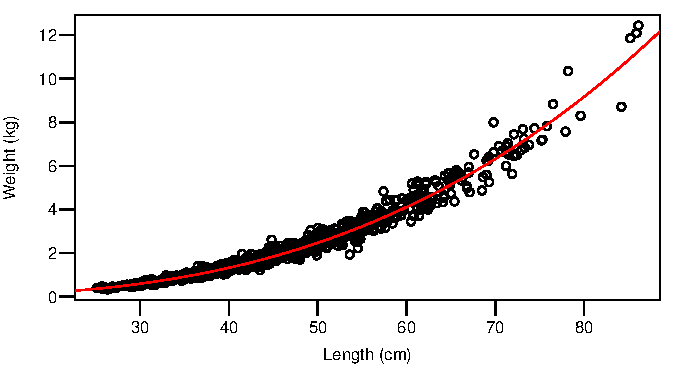
\includegraphics{figure/RC-H07-016}
\end{figure}

\end{frame}


\begin{frame}[fragile]
\frametitle{Weight of snapper as a function of length\ldots}
\framesubtitle{Estimated weight of a 30cm snapper}

Recall that we wanted to estimate the weight of 30 cm snapper.
Since the linear model is fitted to log(wgt), we must back-transform,
and are making inference about median weight.

\begin{knitrout}\scriptsize
\definecolor{shadecolor}{rgb}{0.969, 0.969, 0.969}\color{fgcolor}\begin{kframe}
\begin{alltt}
\hlstd{> }\hlstd{Pred.df}\hlkwb{=}\hlkwd{data.frame}\hlstd{(}\hlkwc{len}\hlstd{=}\hlnum{30}\hlstd{)}
\hlstd{> }\hlkwd{exp}\hlstd{(}\hlkwd{predict}\hlstd{(Snap.lm,Pred.df,}\hlkwc{interval}\hlstd{=}\hlstr{"confidence"}\hlstd{))}
\end{alltt}
\begin{verbatim}
        fit       lwr       upr
1 0.5937602 0.5857844 0.6018445
\end{verbatim}
\end{kframe}
\end{knitrout}
That is, we estimate 30 cm snapper to have median weight between 586 and 602 grams.
\medskip

\textbf{Note:} If the research question had asked up to {\em predict} the weight of a 30 cm 
snapper then we would use
\begin{knitrout}\scriptsize
\definecolor{shadecolor}{rgb}{0.969, 0.969, 0.969}\color{fgcolor}\begin{kframe}
\begin{alltt}
\hlstd{> }\hlkwd{exp}\hlstd{(}\hlkwd{predict}\hlstd{(Snap.lm,Pred.df,}\hlkwc{interval}\hlstd{=}\hlstr{"prediction"}\hlstd{))}
\end{alltt}
\begin{verbatim}
        fit       lwr       upr
1 0.5937602 0.4865954 0.7245262
\end{verbatim}
\end{kframe}
\end{knitrout}
We predict a 30 cm snapper to weigh between about 487 and 725 grams.
\end{frame}


\begin{frame}[fragile]
\frametitle{Weight of snapper as a function of length\ldots}
\framesubtitle{Testing $H_0: \beta_1=3$}

A few slides earlier we deduced that the power coefficient $\beta_1$ should be close to,
though not necessarily equal to 3.\\
\bigskip
Let us examine this formally by testing the null hypothesis $H_0: \beta_1=3$.\\
\bigskip
\textbf{Question 1} Is this hypothesis rejected at the 5\% level?
(Hint: the answer can be worked out from output already seen) \\
\bigskip
\textbf{Question 2} What is the \pval{} for $H_0: \beta_1=3$? (This takes a bit more work).
\bigskip
\end{frame}


\begin{frame}[fragile]
\frametitle{What is the \pval{}?}
\begin{knitrout}\scriptsize
\definecolor{shadecolor}{rgb}{0.969, 0.969, 0.969}\color{fgcolor}\begin{kframe}
\begin{alltt}
\hlstd{> }\hlstd{beta1} \hlkwb{=} \hlkwd{coef}\hlstd{(Snap.lm)[}\hlnum{2}\hlstd{]}
\hlstd{> }\hlstd{seBeta1} \hlkwb{=} \hlkwd{summary}\hlstd{(Snap.lm)}\hlopt{$}\hlstd{coefficients[}\hlnum{2}\hlstd{,}\hlnum{2}\hlstd{]}
\hlstd{> }\hlstd{hyp} \hlkwb{=} \hlnum{3}
\hlstd{> }\hlstd{tstat} \hlkwb{=} \hlstd{(beta1} \hlopt{-} \hlstd{hyp)}\hlopt{/}\hlstd{seBeta1}
\hlstd{> }\hlstd{tstat}
\end{alltt}
\begin{verbatim}
 log(len) 
-14.22257 
\end{verbatim}
\begin{alltt}
\hlstd{> }\hlstd{pval} \hlkwb{=} \hlnum{2} \hlopt{*} \hlstd{(}\hlnum{1} \hlopt{-} \hlkwd{pt}\hlstd{(}\hlkwd{abs}\hlstd{(tstat),} \hlkwc{df} \hlstd{=} \hlkwd{nrow}\hlstd{(Snap.df)} \hlopt{-} \hlnum{2}\hlstd{))}
\hlstd{> }\hlstd{pval}
\end{alltt}
\begin{verbatim}
log(len) 
       0 
\end{verbatim}
\end{kframe}
\end{knitrout}
The \pval{} is so small that it been rounded down to zero.

If we really want to see the \pval{} then we can get the \rcode{pt} function 
to do the probability calculation on the log scale, and then exponentiate:\footnote{Not examinable}

\begin{knitrout}\scriptsize
\definecolor{shadecolor}{rgb}{0.969, 0.969, 0.969}\color{fgcolor}\begin{kframe}
\begin{alltt}
\hlstd{> }\hlstd{logP} \hlkwb{=} \hlkwd{log}\hlstd{(}\hlnum{2}\hlstd{)}\hlopt{+}\hlkwd{pt}\hlstd{(}\hlopt{-}\hlkwd{abs}\hlstd{(tstat),} \hlkwc{df} \hlstd{=} \hlkwd{nrow}\hlstd{(Snap.df)} \hlopt{-} \hlnum{2}\hlstd{,} \hlkwc{log.p} \hlstd{= T)}
\hlstd{> }\hlkwd{exp}\hlstd{(logP)}
\end{alltt}
\begin{verbatim}
    log(len) 
2.677086e-41 
\end{verbatim}
\end{kframe}
\end{knitrout}
We see that the \pval() is in the order of $10^{-41}$, i.e., virtually zero.\footnote{By way of comparison, the earth has about $10^{50}$ atoms.}

\end{frame}


%%%%%%%%%%%%%%%%%%%%%%%%%%%%%%%%%%%%%%%%%%%%%%%%%%%%%%%%%%%%%%%%%%%%%%%%%%%%%%%%%%%%%%%%%%%
\BeginSection{Power law curves and their interpretation}
%%%%%%%%%%%%%%%%%%%%%%%%%%%%%%%%%%%%%%%%%%%%%%%%%%%%%%%%%%%%%%%%%%%%%%%%%%%%%%%%%%%%%%%%%%%


\begin{frame}[fragile]
\frametitle{Power law relationships}
\framesubtitle{Other examples of power curves}
\begin{knitrout}\scriptsize
\definecolor{shadecolor}{rgb}{0.969, 0.969, 0.969}\color{fgcolor}
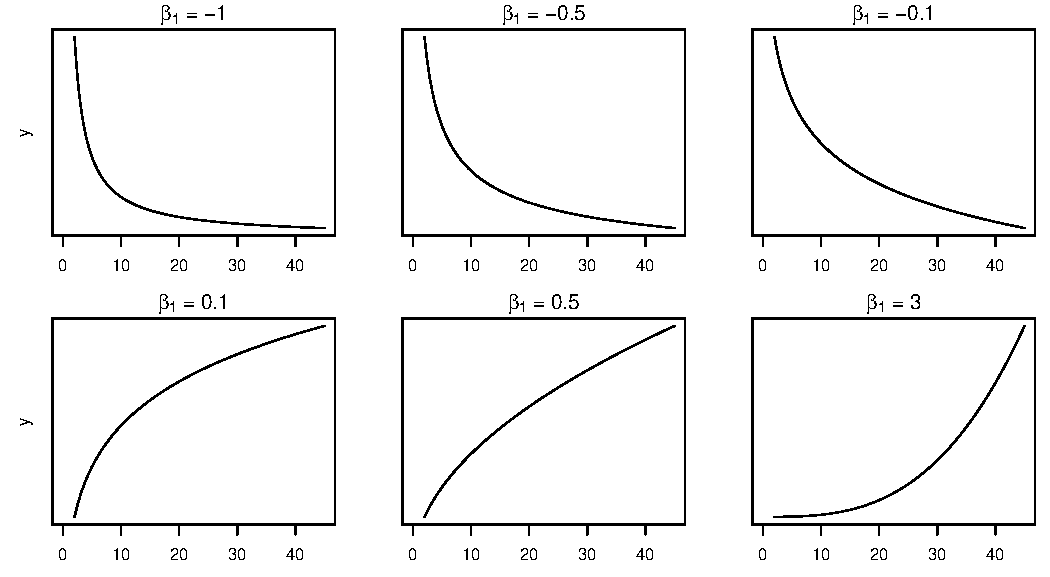
\includegraphics[width=\maxwidth]{figure/RC-H07-020-1} 
\end{knitrout}
In general, 
a power law model could be used whenever one has good reason to believe that the
relationship between $x$ and $y$ takes any of these forms.
\end{frame}


\begin{frame}[fragile]
\frametitle{Power relationships\ldots}
\framesubtitle{Interpretation of power curves}
Recall, we are fitting the model 
$\log(y)=\beta_0+\beta_1 \log(x)$, which is equivalent to
$y=e^{\beta_0}x^{\beta_1} =\alpha x^{\beta_1}$.

\medskip

For the snapper example the confidence interval for $\beta_1$ is 
\begin{knitrout}\scriptsize
\definecolor{shadecolor}{rgb}{0.969, 0.969, 0.969}\color{fgcolor}\begin{kframe}
\begin{alltt}
\hlstd{> }\hlkwd{confint}\hlstd{(Snap.lm)[}\hlnum{2}\hlstd{,]}
\end{alltt}
\begin{verbatim}
   2.5 %   97.5 % 
2.762204 2.819879 
\end{verbatim}
\end{kframe}
\end{knitrout}

One way to interpret this is to say that a 1\% increase in the $x=len$ value 
results in a 2.76\% to a 2.82\% increase in the median value of $y=wgt$.

\medskip

\textbf{Explanation:} Increasing $x$ by 1\% is the same as multiplying $x$ by 1.01.
So the  relative change in $y$ is: 

\vspace{-0.5em}

\[
\Delta y=\frac{\alpha (1.01x)^{\beta_1}}{\alpha x^{\beta_1}}
=\frac{\alpha x^{\beta_1}(1.01)^{\beta_1}}{\alpha x^{\beta_1}}=1.01^{\beta_1}
\]

\vspace{-1em}

$1.01^{\beta_1}\approx 1+\beta_1\times .01$ for reasonable values of $\beta_1$  (Taylor's series).
So, a 1\% increase in $x$ results in an approximate relative increase in $y$ of  $\Delta y\approx \beta_1\times .01$ or an increase of $\beta_1\%$
\end{frame}


\begin{frame}[fragile]
\frametitle{Power relationships\ldots}
\framesubtitle{Interpretation of power curves\ldots}
Alternatively, it might be more meaningful to quantify the change in the median of $y$ arising from a 50\% increase in $x$, or perhaps a doubling of $x$, say 50\% increase in $x$: Then $y$ changes from $\alpha x^{\beta_1}$ to 

\[ \alpha (1.5x)^{\beta_1} =  \alpha x^{\beta_1} 1.5^{\beta_1} \]

i.e., the median of $y$ gets multiplied by $1.5^{\beta_1}$. \\

\bigskip

Doubling in $x$: Then $y$ changes from $\alpha x^{\beta_1}$ to 
\[ \alpha (2x)^{\beta_1} =  \alpha x^{\beta_1} 2^{\beta_1} \]
i.e., the median of $y$ gets multiplied by $2^{\beta_1}$.
\end{frame}


\begin{frame}[fragile]
\frametitle{Power relationships\ldots}
\framesubtitle{Interpretation of power curves\ldots}

\begin{knitrout}\scriptsize
\definecolor{shadecolor}{rgb}{0.969, 0.969, 0.969}\color{fgcolor}\begin{kframe}
\begin{alltt}
\hlstd{> }\hlnum{1.5}\hlopt{^}\hlkwd{confint}\hlstd{(Snap.lm)[}\hlnum{2}\hlstd{,]}
\end{alltt}
\begin{verbatim}
   2.5 %   97.5 % 
3.064785 3.137300 
\end{verbatim}
\end{kframe}
\end{knitrout}
That is, increasing length by 50\% corresponds to an increase in median
snapper weight between 206\% and 214\%\footnote{These percentages are given by \rcode{100*(1.5\^{}confint(Snap.lm)[2,]-1)}.}.
\footnote{One could also say that median snapper weight is between 2.06 and 2.14 times higher. Be careful {\bf not} to say that it is between 3.06 and 3.14 times higher (since it actually multiplies by between 3.06 and 3.14). It is probably safest to talk about \% change.}

\vspace{7mm}
\begin{knitrout}\scriptsize
\definecolor{shadecolor}{rgb}{0.969, 0.969, 0.969}\color{fgcolor}\begin{kframe}
\begin{alltt}
\hlstd{> }\hlnum{2}\hlopt{^}\hlkwd{confint}\hlstd{(Snap.lm)[}\hlnum{2}\hlstd{,]}
\end{alltt}
\begin{verbatim}
   2.5 %   97.5 % 
6.784319 7.061030 
\end{verbatim}
\end{kframe}
\end{knitrout}
That is, doubling length corresponds to an increase in median
weight between 578\% and 606\%.

\end{frame}


%%%%%%%%%%%%%%%%%%%%%%%%%%%%%%%%%%%%%%%%%%%%%%%%%%%%%%%%%%%%%%%%%%%%%%%%%%%%%%%%%%%%%%%%%%%
\BeginSection{Relevant \rcode{R}-code}
%%%%%%%%%%%%%%%%%%%%%%%%%%%%%%%%%%%%%%%%%%%%%%%%%%%%%%%%%%%%%%%%%%%%%%%%%%%%%%%%%%%%%%%%%%%


\begin{frame}[fragile]
\frametitle{Most of the \rcode{R}-code you need for this chapter}

When your response variable is right skew and you have a good reason to believe the underlying relationship follows a power relationship then try taking logs of both $y$ and $x$.

\begin{knitrout}\scriptsize
\definecolor{shadecolor}{rgb}{0.969, 0.969, 0.969}\color{fgcolor}\begin{kframe}
\begin{alltt}
\hlstd{> }\hlstd{Snap.lm}\hlkwb{=}\hlkwd{lm}\hlstd{(}\hlkwd{log}\hlstd{(wgt)}\hlopt{~}\hlkwd{log}\hlstd{(len),}\hlkwc{data}\hlstd{=Snap.df)}
\end{alltt}
\end{kframe}
\end{knitrout}
\medskip

We state the effect as the \% change in the median of $y$ for a given \% change in $x$.
\bigskip

The confidence interval for $\beta_1$ is 
\begin{knitrout}\scriptsize
\definecolor{shadecolor}{rgb}{0.969, 0.969, 0.969}\color{fgcolor}\begin{kframe}
\begin{alltt}
\hlstd{> }\hlkwd{confint}\hlstd{(Snap.lm)[}\hlnum{2}\hlstd{,]}
\end{alltt}
\end{kframe}
\end{knitrout}
and is the (approximate) \% change in the median $y$ for a 1\% increase in $x$.
\medskip

In general, for a $z$\% increase in $x$, the multiplier for the median of $y$ is
\begin{knitrout}\scriptsize
\definecolor{shadecolor}{rgb}{0.969, 0.969, 0.969}\color{fgcolor}\begin{kframe}
\begin{alltt}
\hlstd{> }\hlstd{(}\hlnum{1}\hlopt{+}\hlstd{z}\hlopt{/}\hlnum{100}\hlstd{)}\hlopt{^}\hlkwd{confint}\hlstd{(Snap.lm)[}\hlnum{2}\hlstd{,]}
\end{alltt}
\end{kframe}
\end{knitrout}
or alternatively, the percentage change in the median of $y$ is
\begin{knitrout}\scriptsize
\definecolor{shadecolor}{rgb}{0.969, 0.969, 0.969}\color{fgcolor}\begin{kframe}
\begin{alltt}
\hlstd{> }\hlnum{100}\hlopt{*}\hlstd{((}\hlnum{1}\hlopt{+}\hlstd{z}\hlopt{/}\hlnum{100}\hlstd{)}\hlopt{^}\hlkwd{confint}\hlstd{(Snap.lm)[}\hlnum{2}\hlstd{,]}\hlopt{-}\hlnum{1}\hlstd{)}
\end{alltt}
\end{kframe}
\end{knitrout}

\end{frame}

\end{document}



